\chapter{Loop closure and place recognition}
\label{ch:loop}

In Chapter~\ref{ch:posegraph} the loop closures were given to us: we
knew which keyframes saw the same landmarks because the simulation
told us. A real system has only images. It must recognise, from
appearance alone, that the place it sees now is a place it has seen
before, among hundreds or thousands of keyframes, in a few
milliseconds; and it must then measure the relative pose between the
two keyframes accurately enough to become a factor of the pose graph.
The first task is \emph{place recognition}, an image retrieval problem;
the second is \emph{geometric verification}, a small bundle adjustment.
This chapter builds both, finds the loops of our garden from simulated
descriptors, and then looks closely at the loops that pass every test
and are still wrong.

\section{Place recognition}

\begin{definition}{Place recognition}{placerec}
Given a database of keyframes $I_1,\dots,I_{j-1}$ and a query keyframe
$I_j$, find the keyframes $I_i$ that see a substantial part of the
scene seen by $I_j$. In SLAM the recent keyframes $i>j-g$ are excluded
($g$ is the \emph{minimum gap}): they trivially look like $I_j$, and
the local bundle adjustment already links them.
\end{definition}

Two kinds of error are possible, and they are not equally bad. A missed
loop (a false negative) costs accuracy: the drift is corrected later,
or not at all. A wrong loop (a false positive) adds a factor that
claims two distant places are the same; Section~\ref{sec:pgrobust}
showed that one such factor can bend a whole least-squares map.
Place recognition is therefore tuned for precision first, and recall
second.

Matching the descriptors of $I_j$ against those of every earlier
keyframe would work, but its cost grows with the number of keyframes
times the square of the number of features: with 300 features per
keyframe and a few thousand keyframes after a season of mowing, that is
some $10^8$ Hamming distances per query. The standard answer, borrowed
from text retrieval, is to describe each image by the \emph{words} it
contains.

\section{A vocabulary of binary words}

\begin{definition}{Visual vocabulary}{vocab}
A vocabulary is a set of $k$ binary strings $\vect{c}_1,\dots,
\vect{c}_k\in\{0,1\}^n$, the \emph{words}. It quantises a descriptor
$\vect{d}$ to the index of its nearest word, $q(\vect{d})=
\arg\min_w d_H(\vect{d},\vect{c}_w)$, with $d_H$ the Hamming distance.
The set of descriptors with the same word is a Voronoi cell of
$\{0,1\}^n$.
\end{definition}

The words are learnt offline by clustering a large set of training
descriptors. For real-valued descriptors this is $k$-means; for binary
ones the mean is replaced by a bitwise majority vote.

\begin{proposition}{$k$-majority}{kmaj}
Let $\vect{d}_1,\dots,\vect{d}_N\in\{0,1\}^n$, and consider the cost
\begin{equation}\label{eq:kmajcost}
C(\vect{c}_{1:k},\ell)=\sum_{a=1}^N d_H\bigl(\vect{d}_a,
\vect{c}_{\ell(a)}\bigr)
\end{equation}
of centres $\vect{c}_w$ and labels $\ell(a)\in\{1,\dots,k\}$.
\begin{enumerate}[nosep]
\item For a fixed cluster $A=\{a:\ell(a)=w\}$, the bitwise majority
  $c_{w,b}=[\,|\{a\in A:d_{a,b}=1\}|>|A|/2\,]$ minimises $\sum_{a\in A}
  d_H(\vect{d}_a,\vect{c})$ over $\vect{c}\in\{0,1\}^n$.
\item Alternating the assignment $\ell(a)=q(\vect{d}_a)$ and the
  majority update never increases $C$, and the algorithm reaches a
  fixed point in finitely many steps.
\end{enumerate}
\end{proposition}

\begin{proof}
1. The Hamming distance is a sum over bits, $d_H(\vect{d},\vect{c})=
\sum_b[d_b\neq c_b]$, so $\sum_{a\in A}d_H(\vect{d}_a,\vect{c})=
\sum_b\sum_{a\in A}[d_{a,b}\neq c_b]$ and each bit $c_b$ can be chosen
independently. If $m_b$ members have $d_{a,b}=1$, choosing $c_b=1$
costs $|A|-m_b$ and $c_b=0$ costs $m_b$; the majority picks the
smaller (either, on a tie).

2. With the centres fixed, assigning each descriptor to its nearest
centre minimises each term of \eqref{eq:kmajcost} separately, so $C$
does not increase. With the labels fixed, $C$ is a sum over clusters,
and by part~1 the majority minimises each; an empty cluster contributes
nothing whatever its centre, so re-seeding it does not change $C$.
Hence $C$ is non-increasing. It takes values in the non-negative
integers, so it can strictly decrease only finitely many times;
if ties are broken consistently (keep the current label and the current
bit), an iteration that does not decrease $C$ changes nothing, which is
a fixed point. (\code{bow.kmajority} sets a tied bit to $0$ and simply
runs a fixed number of iterations.)
\end{proof}

Like $k$-means, $k$-majority finds a local minimum that depends on the
initial centres. Real systems use a \emph{vocabulary tree}: cluster
into $k_1$ words, cluster each cell again, and so on for $L$ levels.
DBoW2, used by ORB-SLAM, has $k_1=10$ and $L=6$: a million words, and
quantising a descriptor takes $k_1L=60$ distance computations instead
of a million. Our garden needs far fewer words, and \code{vslam/bow.py}
uses a flat vocabulary of 500.

\section{Bags of words and their similarity}

\begin{definition}{tf-idf vector}{tfidf}
Let image $I$ have $n_I$ descriptors, $n_{I,w}$ of which quantise to
word $w$, and let $N_w$ of the $N$ training images contain $w$. The
\emph{term frequency} is $\mathrm{tf}_{I,w}=n_{I,w}/n_I$, the
\emph{inverse document frequency} $\mathrm{idf}_w=\log(N/N_w)$, and the
bag-of-words vector of $I$ is
\begin{equation}\label{eq:tfidf}
\vect{v}_I=\frac{\vect{u}}{\norm{\vect{u}}_1},\qquad
u_w=\mathrm{tf}_{I,w}\,\mathrm{idf}_w .
\end{equation}
\end{definition}

A word present in every training image has $\mathrm{idf}=0$: seeing it
says nothing about where one is. The idf is the self-information
$-\log P(w\in I)$ of the event ``an image contains $w$'', estimated on
the training set: rare words carry more information, and they get more
weight.

\begin{proposition}{The $L_1$ score}{lonescore}
For vectors $\vect{v},\vect{w}\ge0$ with $\norm{\vect{v}}_1=
\norm{\vect{w}}_1=1$, the DBoW2 score
\begin{equation}\label{eq:score}
s(\vect{v},\vect{w})=1-\tfrac12\norm{\vect{v}-\vect{w}}_1
=\sum_{k}\min(v_k,w_k)
\end{equation}
lies in $[0,1]$; it equals $1$ if and only if $\vect{v}=\vect{w}$, and
$0$ if and only if $\vect{v}$ and $\vect{w}$ have no non-zero entry in
common. Only the words present in both images contribute to it.
\end{proposition}

\begin{proof}
For reals $a,b$, $|a-b|=a+b-2\min(a,b)$. Summing over $k$ and using
$\sum v_k=\sum w_k=1$ gives $\norm{\vect{v}-\vect{w}}_1=2-2\sum_k
\min(v_k,w_k)$, which is \eqref{eq:score}. Each $\min(v_k,w_k)$ lies in
$[0,v_k]$, so $0\le s\le\sum v_k=1$. The score
is $1$ iff $\min(v_k,w_k)=v_k$ for all $k$, i.e.\ $\vect{w}\ge\vect{v}$
entrywise; since both sum to $1$, this forces $\vect{v}=\vect{w}$. It is
$0$ iff every $\min(v_k,w_k)$ vanishes, i.e.\ no word has non-zero weight
in both. A word absent from either image has $\min=0$.
\end{proof}

The last property is what makes retrieval fast. An \emph{inverted
index} stores, for each word, the list of keyframes containing it with
their weights. To score a query one walks only the lists of the query's
words and accumulates $\min(v_k,w_k)$ per keyframe: keyframes sharing no
word with the query are never touched. (\code{vslam/bow.py} uses dense
vectors for clarity; with 153 keyframes and 500 words that is fast
enough.)

Raw scores are hard to threshold: the score between two views of the
same place depends on how textured the place is and how fast the camera
moves. DBoW2 normalises by the score of the query with its predecessor,
\begin{equation}\label{eq:normscore}
\eta(j,i)=\frac{s(\vect{v}_j,\vect{v}_i)}{s(\vect{v}_j,\vect{v}_{j-1})},
\end{equation}
the score one can expect for ``the same place'' here and now. A
candidate with $\eta$ near or above $1$ looks as much like $I_j$ as
$I_{j-1}$ does.

\begin{figure}[ht]
\centering
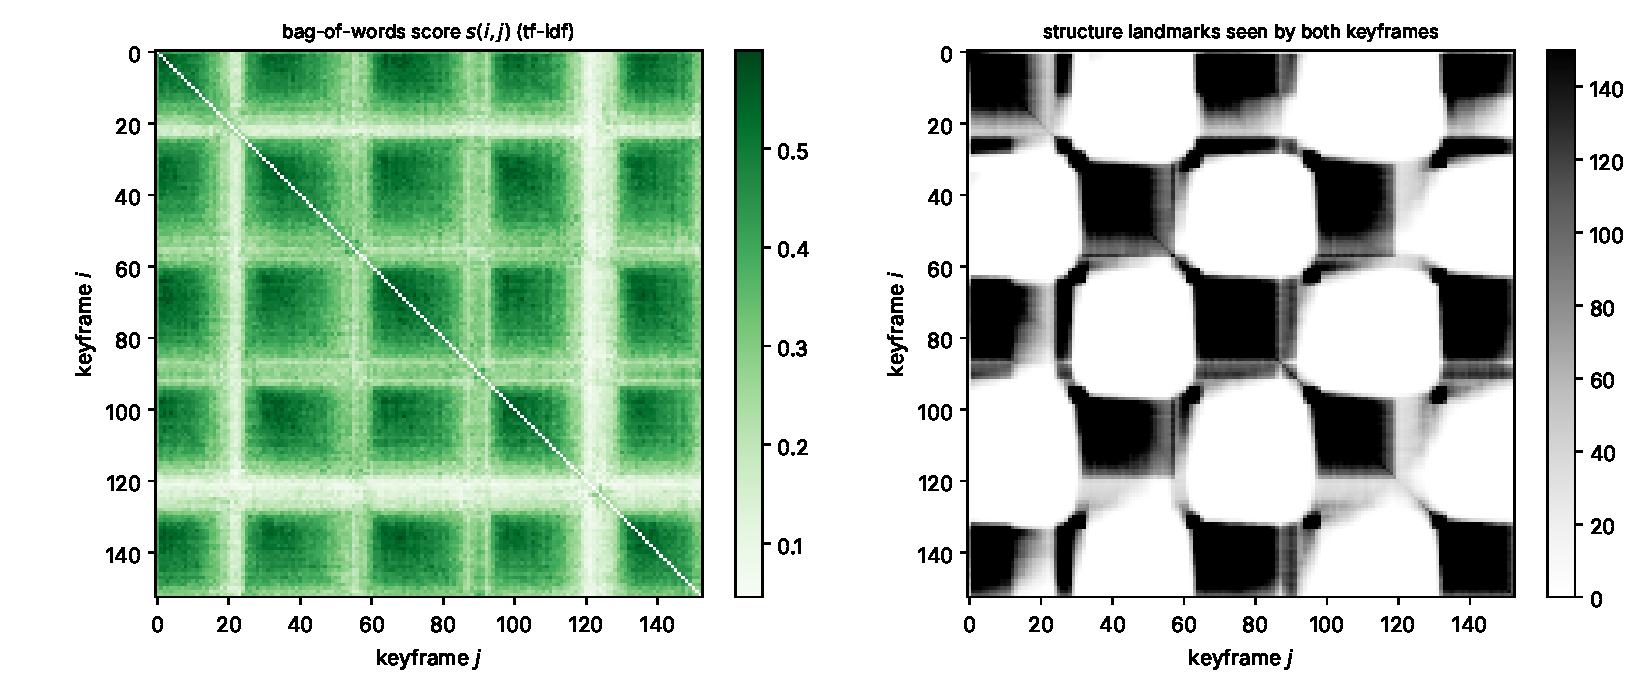
\includegraphics[width=\linewidth]{figures/ch10_similarity.pdf}
\caption{Left: tf-idf scores between the 153 keyframes of the garden
run (vocabulary of 500 words learnt on a different garden). Right: the
number of structure landmarks seen by both keyframes. The block pattern
is the mowing pattern: rows in the same direction look at the same
fence, house and trees.}
\label{fig:similarity}
\end{figure}

\section{Simulated appearance and aliasing}

The garden simulation of the previous chapters has geometry but no
images. To exercise place recognition, \code{sim.landmark\_descriptors}
gives every landmark a 256-bit base descriptor, and
\code{sim.observe\_descriptors} flips a fraction of its bits at every
observation (viewpoint, light, wind): 8\,\% for structure, 15\,\% for
grass. The house, the shed and the trees get independent random
descriptors. Fence pickets and grass patches do not: each copies one of
a few \emph{prototypes} (40 for the fence, 15 for the grass) with only
4\,\% of its bits changed. Repetitive structure that looks the same
everywhere is called \emph{perceptual aliasing}, and it is the main
enemy of place recognition outdoors.

\begin{lemma}{Distance between perturbed strings}{hamperturb}
Let $\vect{d},\vect{d}'\in\{0,1\}^n$ be obtained from the same string by
flipping each bit independently with probability $r$ (independently for
$\vect{d}$ and $\vect{d}'$). Then $d_H(\vect{d},\vect{d}')\sim
\mathrm{Binomial}(n,2r(1-r))$. Two independent uniform random strings
are at distance $\mathrm{Binomial}(n,\frac12)$.
\end{lemma}

\begin{proof}
Bit $b$ differs if exactly one of the two copies flipped it, with
probability $r(1-r)+(1-r)r$, independently across bits; the distance is
the number of differing bits. For random strings each bit differs with
probability $\frac12$.
\end{proof}

\begin{example}{How alike two pickets are}{pickets}
Two observations of the same picket: $r=0.08$, distance
$\mathrm{B}(256,0.147)$, mean $37.7$, standard deviation $5.7$. Two
pickets of the same prototype: each differs from the prototype by its
personal 4\,\% and an observation's 8\,\%, a net flip probability
$r=0.04\cdot0.92+0.96\cdot0.08=0.114$, hence mean $256\cdot2r(1-r)=
51.6$, standard deviation $6.4$. Two unrelated landmarks: mean $128$,
standard deviation $8$. With 2\,\% personal bits instead of 4\,\%,
$r=0.097$ and the second mean drops to $44.8$.
\end{example}

The two distributions overlap. A picket is often almost as close to
another picket as to itself, and Lowe's ratio test
(\cref{def:matching}) then rejects the match as ambiguous (Exercise
\ref{ex:10ratio}). Aliasing therefore acts in two ways: it makes images
of different places score alike, and it removes the matches on the
repetitive structure, leaving the verification with fewer and less
well-spread correspondences. The second effect turns out to be the
dangerous one.

\begin{figure}[ht]
\centering
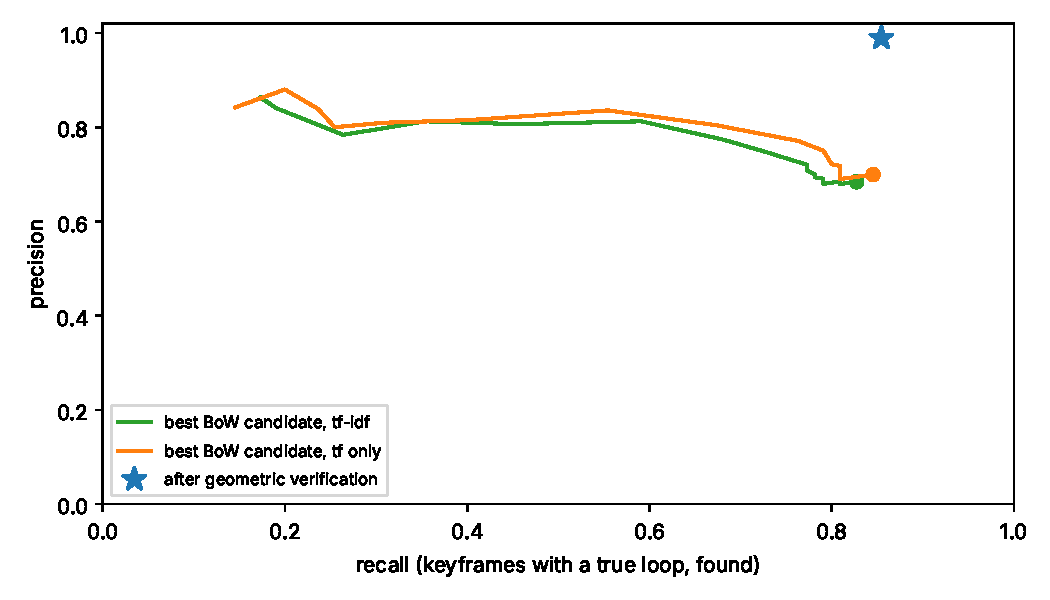
\includegraphics[width=0.75\linewidth]{figures/ch10_pr.pdf}
\caption{Precision and recall of the best bag-of-words candidate of
each keyframe, as the threshold on the normalised score
\eqref{eq:normscore} varies (dots: the threshold 0.6 used by the
detector). A candidate is counted as correct if it shares at least 30
structure landmarks with the query; 110 of the 153 keyframes have such
a partner at least 20 keyframes back. Star: the loops accepted after
geometric verification.}
\label{fig:pr}
\end{figure}

\Cref{fig:pr} shows what appearance alone achieves: about 70\,\% of
the best candidates are correct at a recall above 80\,\%. That is far
too many wrong loops to give to a pose graph, but a very useful
shortlist. The idf weighting makes no difference here, because the
simulated descriptors are random and no word is much more common than
another; on real images, where some words (grass texture, the edge of
the sky) occur everywhere, it matters.

\section{Geometric verification}

The shortlist is checked by geometry: do the matched features of $I_i$
and $I_j$ agree with \emph{one} rigid motion? And if they do, what is
it, with what uncertainty? This relative pose $Z_{ij}=T_i^{-1}T_j$
becomes the loop factor.

The obvious method is the one of the VO (Chapter~\ref{ch:vo}):
triangulate the stereo points of $I_i$ and run PnP against the features
of $I_j$. Between neighbouring lawn rows it fails. The landmarks that
the two keyframes share are the far ones --- the fence across the lawn,
the trees and the house beyond, 9 to 15\,m away --- and one stereo pair
with a 12\,cm baseline triangulates them badly. By \eqref{eq:depthstd}
with $\sigma_\delta=\sqrt2\cdot0.5$\,px, a point at 10\,m has
$\sigma_Z\approx1.3$\,m. Seen from a keyframe displaced sideways by
$d=3$\,m, a depth error $\Delta Z$ moves its image by about
$f\,\Delta Z\,d/Z^2\approx18$\,px: PnP inliers and outliers can no
longer be told apart, and the pose is metres off.

The verification in \code{vslam/loop.py} therefore uses the depths only
where they are reliable:
\begin{enumerate}[nosep]
\item Match the descriptors of $I_i$ (points with a usable stereo depth)
  and $I_j$, with the ratio test and the mutual check.
\item Five-point RANSAC on the normalised coordinates
  (\cref{thm:essential}, threshold $1.5\sigma/f$): bearings only, so the
  depth errors play no role in selecting the inliers.
\item Decompose $E$ into $R$ and the direction $\hat{\vect{t}}$
  (\cref{prop:decompose}), and recover the scale from both keyframes'
  stereo points (\cref{prop:stereoscale}).
\item A bundle adjustment of the two keyframes and the inlier points,
  with the stereo measurements of both (Cauchy kernel, $T_i$ fixed). A
  loop is accepted if at least 25 points have a small residual in both
  keyframes.
\item The covariance of $Z_{ij}$ is that of the BA (\cref{prop:bacov}),
  inflated by four as in Chapter~\ref{ch:posegraph}.
\end{enumerate}

\begin{proposition}{Scale from two stereo keyframes}{stereoscale}
Let $\vect{q}^A_a$ and $\vect{q}^B_a$ be the stereo points of match $a$
in keyframes $A$ and $B$, and let $\vect{q}^B=R\vect{q}^A+s\hat{\vect{t}}$
with $R$, $\hat{\vect{t}}$ known and $\norm{\hat{\vect{t}}}=1$. The
least-squares scale is
\begin{equation}\label{eq:stereoscale}
\hat s=\arg\min_s\sum_a\norm{\vect{q}^B_a-R\vect{q}^A_a-s\hat{\vect{t}}}^2
=\frac1m\sum_{a=1}^m\hat{\vect{t}}\T\bigl(\vect{q}^B_a-R\vect{q}^A_a\bigr).
\end{equation}
\end{proposition}

\begin{proof}
The cost is a quadratic in $s$ with derivative $-2\sum_a\hat{\vect{t}}\T
(\vect{q}^B_a-R\vect{q}^A_a-s\hat{\vect{t}})$; setting it to zero and using
$\hat{\vect{t}}\T\hat{\vect{t}}=1$ gives \eqref{eq:stereoscale}.
\end{proof}

Each term of \eqref{eq:stereoscale} is noisy (metres, for far points),
but the noise averages over a hundred matches, and the code takes the
median to resist a few bad depths. The bundle adjustment then does what
no single keyframe can: it triangulates each matched point from two
stereo pairs whose separation is the metres between the keyframes, not
the 12\,cm of the rig.

\begin{inwords}
Choose the correspondences with the measurements you trust (bearings),
start the pose from them, and only then let the less trusted ones
(single-keyframe depths) take part, inside an optimisation that can
re-estimate them. The first version of our verification started the BA
from the PnP pose instead: on far points that pose was 2--4\,m off, and
about one loop in ten converged to a wrong answer although every inlier
match was correct. Starting from the five-point pose removed almost all
of them.
\end{inwords}

\section{Loops that are still wrong}
\label{sec:wrongloops}

\begin{figure}[t]
\centering
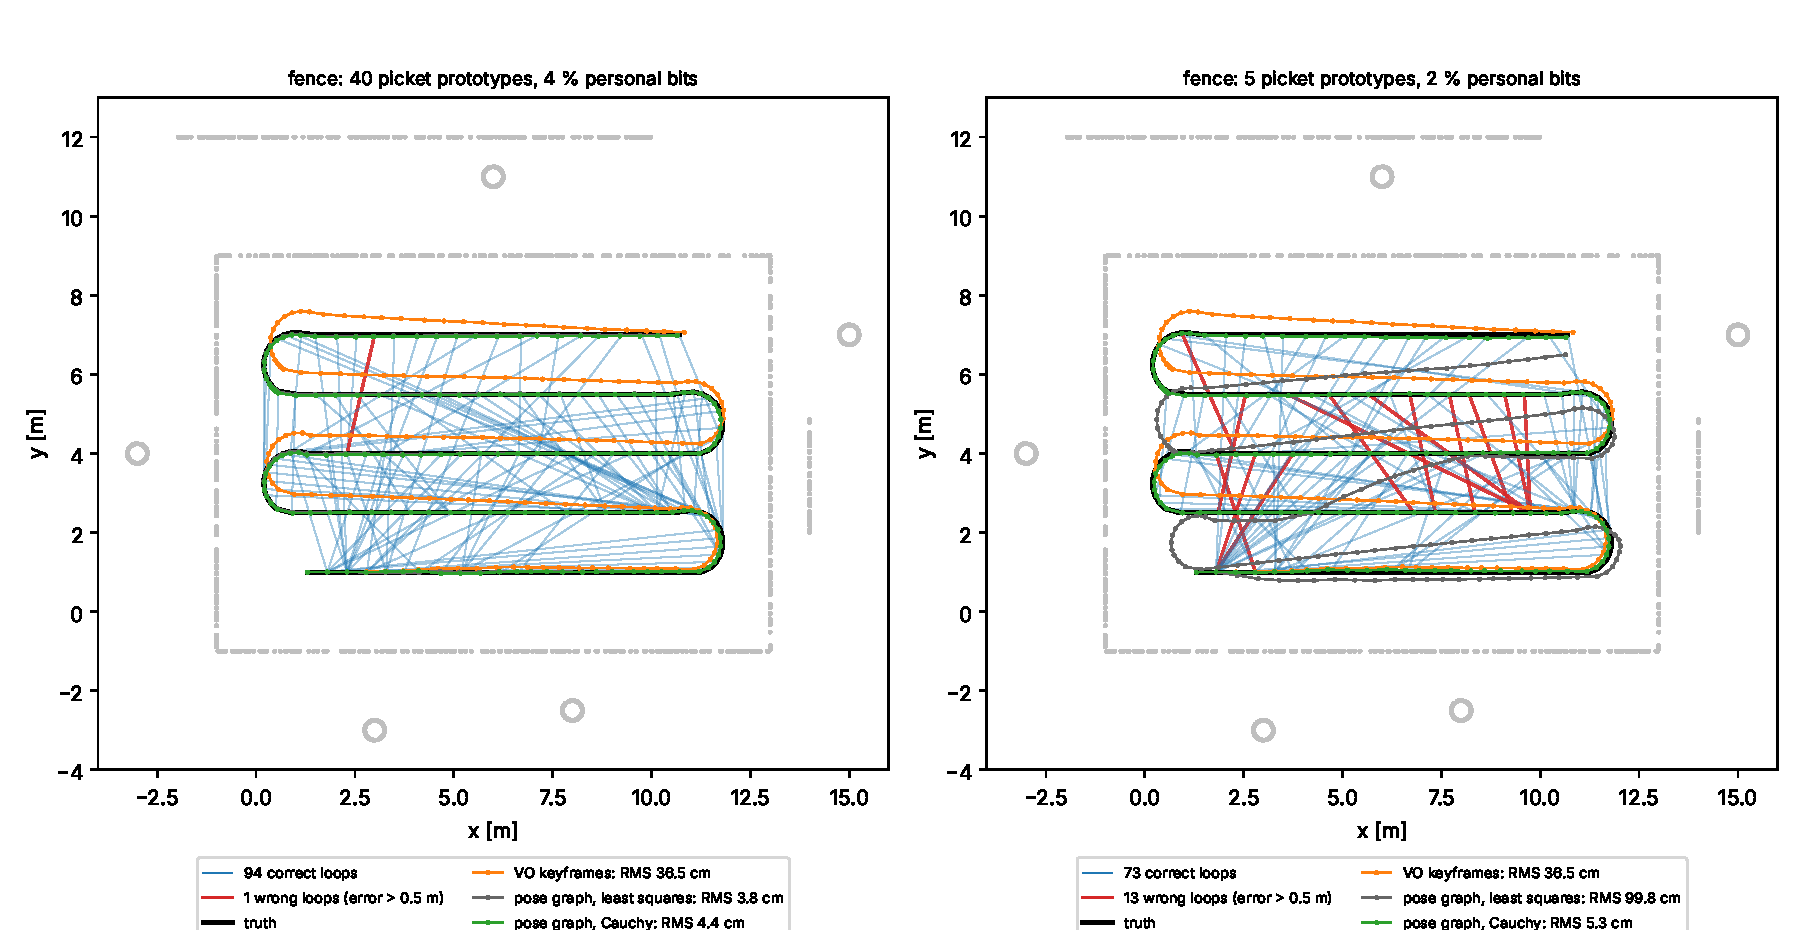
\includegraphics[width=\linewidth]{figures/ch10_loops.pdf}
\caption{Loops found from the simulated descriptors and the pose graph
of Chapter~\ref{ch:posegraph} (odometry factors $2$\,cm, $0.23^\circ$)
corrected with them. Left: the default garden. Right: a fence of only 5
picket prototypes with 2\,\% personal bits. A loop is drawn red if its
translation is more than 0.5\,m wrong. Each wrong loop's inlier
matches are all correct.}
\label{fig:loops}
\end{figure}

In the default garden, the detector accepts 95 loops; the median error
of their translations is 6\,cm and one is wrong (0.54\,m), and the pose
graph brings the VO's 36.5\,cm RMS error down to 3.8\,cm with least
squares and 4.4\,cm with a Cauchy kernel --- the level of the oracle
loops of Chapter~\ref{ch:posegraph}. With a strongly aliased fence
(\cref{fig:loops}, right) it accepts 86 loops, 13 of them wrong by
0.6--4.6\,m, and least squares ends at a metre of RMS error; the Cauchy
kernel still reaches 5.3\,cm.

The surprise is that the wrong loops have \emph{no} wrong matches. With
the fence matches removed by the ratio test, their inliers lie almost
all on one tree trunk (with part of the shed, for a few), a narrow
object 10 to 15\,m away. The
next two propositions show why that is not enough.

\begin{proposition}{The motion field}{motionfield}
A camera moving with linear velocity $\vect{v}$ and angular velocity
$\bomega$ (both in the camera frame) sees a static point at depth $Z$
and normalised coordinates $(x,y)$ move with
\begin{equation}\label{eq:motionfield}
\begin{aligned}
\dot x&=\frac{-v_x+x\,v_z}{Z}+xy\,\omega_x-(1+x^2)\,\omega_y+y\,\omega_z,\\
\dot y&=\frac{-v_y+y\,v_z}{Z}+(1+y^2)\,\omega_x-xy\,\omega_y-x\,\omega_z.
\end{aligned}
\end{equation}
\end{proposition}

\begin{proof}
In the camera frame the point moves with $\dot{\vect{X}}=-\vect{v}-
\bomega\times\vect{X}$, i.e.\ $\dot X=-v_x-\omega_yZ+\omega_zY$,
$\dot Y=-v_y-\omega_zX+\omega_xZ$, $\dot Z=-v_z-\omega_xY+\omega_yX$.
Differentiate $x=X/Z$: $\dot x=\dot X/Z-x\dot Z/Z$. Substituting, with
$X/Z=x$ and $Y/Z=y$,
$\dot x=-v_x/Z-\omega_y+\omega_zy+x\,v_z/Z+x\,\omega_xy-x\,\omega_yx$,
which is the first line. The second follows in the same way from
$\dot y=\dot Y/Z-y\dot Z/Z$.
\end{proof}

\begin{proposition}{Rotation--translation ambiguity}{rtambig}
Suppose all points satisfy $|x|\le\epsilon_x$, $|y|\le\epsilon_y$ and
$|\bar Z/Z-1|\le\delta$ for some $\bar Z$. Then the motion
$\vect{v}=(-\bar Z\omega,0,0)$, $\bomega=(0,\omega,0)$ --- a sideways
translation and a rotation that compensates it --- moves every point by
at most
\begin{equation}\label{eq:rtambig}
|\dot x|\le|\omega|\,(\delta+\epsilon_x^2),\qquad
|\dot y|\le|\omega|\,\epsilon_x\epsilon_y ,
\end{equation}
whereas the rotation alone moves them by $|\omega|(1+x^2)\ge|\omega|$.
\end{proposition}

\begin{proof}
In \eqref{eq:motionfield} with $v_y=v_z=\omega_x=\omega_z=0$:
$\dot x=\bar Z\omega/Z-(1+x^2)\omega=\omega(\bar Z/Z-1)-x^2\omega$ and
$\dot y=-xy\,\omega$. Bound each term.
\end{proof}

A trunk of 50\,cm at 10\,m spans $\epsilon_x\approx0.025$; its depth
varies by $\delta\approx0.03$. The motion of
\cref{prop:rtambig} then moves its image some thirty times less than
the rotation alone would: an error of $\omega$ in heading is
almost exactly paid for by a sideways error $\bar Z\omega$ in position.
The cost of the two-keyframe BA has a long, nearly flat valley along
this direction, and the minimum found depends on where the optimiser
starts and when it stops. The wrong loops of \cref{fig:loops} sit in
that valley: for the worst one, the heading is off by $26^\circ$
($0.45$\,rad) and the position by $4.6$\,m sideways, a ratio of
$10.3$\,m --- the distance of the tree. Their inliers are many (50 to
115) and their residuals small; only the geometry is poor. And a
Laplace covariance computed at a point far down the valley is no
guide to the error: for two of these loops it claims 2\,cm.

Several remedies exist, and none is complete.
\begin{itemize}[nosep]
\item \emph{Temporal consistency} (DBoW2): accept a loop $(i,j)$ only
  if keyframes near $j$ also close loops near $i$. Here it keeps 64 of
  the 86 loops and 12 of the 13 wrong ones: the neighbours of $j$ see
  the same tree from nearly the same place and fail in the same way.
\item \emph{Spread}: require the inliers to cover the image. On our
  runs the spread of the wrong loops' inliers overlaps that of many
  correct ones, so a threshold that removes the former also removes
  the latter.
\item \emph{Gating against the current estimate}: compare $Z_{ij}$ with
  the relative pose predicted by the pose graph, using the predicted
  covariance. This catches errors larger than the drift, not the
  half-metre ones.
\item \emph{A robust back-end}: the Cauchy kernel of
  Section~\ref{sec:pgrobust}, switchable constraints or graduated
  non-convexity. This is what saves the right-hand map of
  \cref{fig:loops}.
\end{itemize}
The lesson is the one of Chapter~\ref{ch:posegraph}: the front-end
cannot be made perfect, so the back-end must not believe it blindly.

\section{Scale drift and $\mathrm{Sim}(3)$}

Our stereo rig measures metric depth, so the relative pose of a loop is
in $\SE3$. A monocular system knows the scale only up to the drift
of Chapter~\ref{ch:vo}, and its map at the end of a loop may be at a
different scale from the map at the start.

\begin{definition}{$\mathrm{Sim}(3)$}{sim3}
The similarity transformations of $\R^3$, $S=\bigl(\begin{smallmatrix}
sR&\vect{t}\\0&1\end{smallmatrix}\bigr)$ with $s>0$, $R\in\SO3$,
$\vect{t}\in\R^3$, form a Lie group of dimension 7.
\end{definition}

A monocular loop closure estimates $S_{ij}\in\mathrm{Sim}(3)$ (with
the scaled Umeyama alignment of \cref{prop:umeyama} on the matched
points), and the pose graph is optimised over $\mathrm{Sim}(3)$ so
that the scale correction too is spread along the loop. ORB-SLAM does
exactly this. With stereo (or an IMU, Chapters~12--13) the scale is
observable and $\SE3$ suffices.

\section{Relocalisation}

The same machinery answers a different question: \emph{where am I?}
When tracking is lost (the camera was covered, the mower was lifted and
carried), or when a new mowing session starts in yesterday's map, the
current frame is a query against all keyframes of the map. The best
candidates are verified as above, but now with the map's 3D points,
which the bundle adjustment has triangulated from many keyframes: PnP
against well-known points works (\cref{def:pnp}), and the pose is
then refined by motion-only BA (\cref{def:mba}). Tracking resumes from
there.

\begin{mower}
For the mower, relocalisation is how every session starts: the mower
leaves the shed, recognises the garden and continues in the stored map
rather than building a new one. Two cautions. First, the appearance of
a garden changes over hours (sun and shadows) and seasons (grass height,
leaves); bags of ORB words cope with the former poorly and with the
latter not at all. The structure --- fence, house, shed, trunks --- is
the stable part of the scene, and learnt global descriptors (NetVLAD
and its successors) are far more robust to such changes. Second, the
garden is the worst case of \cref{sec:wrongloops}: long uniform
fences, and a few isolated trees. The RTK-GNSS of Chapter~14 will give
an independent check on every loop.
\end{mower}

\begin{practice}[\code{vslam/bow.py}, \code{vslam/loop.py},
  \code{vslam/sim.py}, \code{examples/ch10\_loops.py},
  \code{notebooks/ch10\_loops.ipynb}]
\begin{center}
\begin{tabular}{@{}ll@{}}
\toprule
Code & Formula\\
\midrule
\code{bow.kmajority} & \cref{prop:kmaj}\\
\code{bow.Vocabulary.train}, \code{.bow} & \cref{def:tfidf}\\
\code{bow.score} & \cref{prop:lonescore}\\
\code{sim.landmark\_descriptors} & \cref{lem:hamperturb}\\
\code{sim.observe\_descriptors} & \cref{lem:hamperturb}\\
\code{loop.LoopDetector.candidates} & \eqref{eq:normscore}\\
\code{loop.LoopDetector.verify} & \cref{prop:stereoscale}, then a BA\\
\code{loop.loop\_edges} & loop factors, BA covariance\\
\bottomrule
\end{tabular}
\end{center}
The tests check that the simulated fence is aliased and the house is
not, that the $k$-majority cost never increases, the properties of the
score, that a word present in every image has zero idf, and that the
verification accepts a true revisit (with a translation error below
30\,cm and a positive definite covariance) and rejects a keyframe pair
that shares too little. The example script produces the figures of this
chapter; the notebook adds the descriptor-distance histograms, the
normalised scores of one keyframe, and a closer look at one loop.
\end{practice}

\section*{Further reading and C++ pointers}
\addcontentsline{toc}{section}{Further reading and C++ pointers}

Bags of words for images: J.~Sivic and A.~Zisserman (ICCV 2003);
vocabulary trees: D.~Nist\'er and H.~Stew\'enius (CVPR 2006); binary
words, the normalised score and temporal consistency: D.~G\'alvez-L\'opez
and J.~D.~Tard\'os (IEEE T-RO 2012). A probabilistic alternative is
FAB-MAP (M.~Cummins and P.~Newman, IJRR 2008); S.~Lowry et~al.\ survey
visual place recognition (IEEE T-RO 2016), and NetVLAD
(R.~Arandjelovi\'c et~al., CVPR 2016) started the learnt global
descriptors. The motion field \eqref{eq:motionfield} is from
H.~C.~Longuet-Higgins and K.~Prazdny (1980). Loop closing over
$\mathrm{Sim}(3)$: H.~Strasdat, J.~M.~M.~Montiel and A.~J.~Davison (RSS
2010) and ORB-SLAM. In C++: DBoW2 and its successor DBoW3, used by
ORB-SLAM2/3; \code{cv::findEssentialMat} and \code{cv::recoverPose} for
steps 2--3; g2o or Ceres for the two-keyframe BA.

\FloatBarrier
\section*{Exercises}
\addcontentsline{toc}{section}{Exercises}

\begin{enumerate}[label=\textbf{10.\arabic*},ref=10.\arabic*]
\item\label{ex:10metric} Show that $1-s(\vect{v},\vect{w})$ is a metric
  on the set of non-negative vectors of unit $L_1$ norm.
\item\label{ex:10ratio} Using the normal approximation of the binomial
  distributions of \cref{ex:pickets}, estimate the probability that the
  ratio test with ratio $0.8$ accepts the correct match of a picket
  when exactly one other picket of the same prototype is in the image.
  Repeat with 2\,\% personal bits.
\item\label{ex:10idf} A word occurs in every image of the test run but
  in few training images (think of grass in a garden, and a vocabulary
  learnt on city streets). What does it do to the scores, and how could
  the idf be adapted online?
\item\label{ex:10motion} For points near the image centre on a plane
  facing the camera at depth $Z$, which two combinations of $(\vect{v},
  \bomega)$ are invisible to first order in \eqref{eq:motionfield}?
  What breaks the ambiguity?
\end{enumerate}

\subsection*{Solutions}

\textbf{10.1.} By \cref{prop:lonescore}, $1-s=\frac12\norm{\vect{v}-
\vect{w}}_1$, half a norm of the difference: it is non-negative,
symmetric, zero only if $\vect{v}=\vect{w}$, and satisfies the triangle
inequality because the $L_1$ norm does. (It is the total variation
distance between the two word distributions.)

\textbf{10.2.} Let $D_1$ be the distance to the correct picket and
$D_2$ to the other one: $D_1\approx\Normal(37.7,5.7^2)$ and
$D_2\approx\Normal(51.6,6.4^2)$, independent. The test accepts when
$D_1<0.8D_2$, i.e.\ when $D_1-0.8D_2<0$, a normal variable of mean
$37.7-41.3=-3.6$ and standard deviation $\sqrt{5.7^2+0.64\cdot6.4^2}=
7.6$: probability $\Phi(3.6/7.6)\approx0.68$. With 2\,\% personal bits,
$D_2\approx\Normal(44.8,6.1^2)$, the mean is $+1.9$, the standard
deviation $7.5$, and the probability $\Phi(-0.25)\approx0.40$. With
several pickets of the same prototype in view, the smallest of their
distances is lower still, and fence matches all but disappear.

\textbf{10.3.} Its idf is large, so it gets a large weight in every
image; two unrelated images of the test run then share a big common
term $\min(v_w,w_w)$, and all scores are pushed up and compressed
together, which hurts the ranking. The normalisation by the
predecessor's score partly compensates. Online, one can recompute the
idf with the keyframes of the map as the document collection, so that
$N_w/N$ reflects the environment being mapped; DBoW2 allows weights to
be computed this way.

\textbf{10.4.} With $x=y=0$ and constant depth, \eqref{eq:motionfield}
reduces to $\dot x=-v_x/Z-\omega_y$, $\dot y=-v_y/Z+\omega_x$, and $v_z$,
$\omega_z$ have no effect at the centre. Invisible at first order:
$(v_x,\omega_y)$ with $v_x=-Z\omega_y$, and $(v_y,\omega_x)$ with
$v_y=Z\omega_x$. (Away from the centre, $v_z$ and $\omega_z$ do show:
they create the expanding and rotating parts of the field.) The
ambiguity is broken by the terms $x^2\omega_y$, $xy\,\omega_x$, \dots,
i.e.\ by a wide field of view, and by a spread of depths, which makes
$v_x/Z$ vary from point to point while $\omega_y$ does not.
